\documentclass[dvipdfmx]{jlreq}

\title{離散数学 レポート課題4}
\author{細川 夏風}
\date{\today}

\usepackage{tikz}
\usepackage{amsmath}
\usepackage{amsfonts}

\begin{document}

\maketitle


\section*{問 1}
\subsection*{無効グラフの例}
\begin{figure}
\begin{centering}
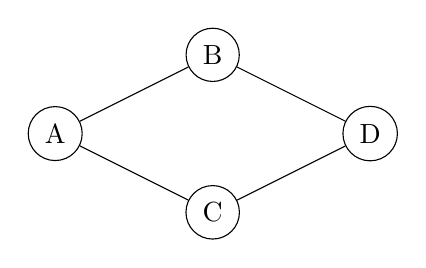
\begin{tikzpicture}
    \node[circle, draw] (A) at (0, 0) {A};
    \node[circle, draw] (B) at (2, 1) {B};
    \node[circle, draw] (C) at (2, -1) {C};
    \node[circle, draw] (D) at (4, 0) {D};

    \draw (A) -- (B);
    \draw (A) -- (C);
    \draw (B) -- (D);
    \draw (C) -- (D);
\end{tikzpicture}
\caption{無向グラフの図}
\end{centering}
\end{figure}

\subsection*{無向グラフの隣接行列}
\[
A = \begin{bmatrix}
0 & 1 & 1 & 0 \\
1 & 0 & 0 & 1 \\
1 & 0 & 0 & 1 \\
0 & 1 & 1 & 0 \\
\end{bmatrix}
\]

\subsection*{無向グラフの隣接リスト}
\begin{itemize}
    \item $A: \rightarrow B \rightarrow C$
    \item $B: \rightarrow A \rightarrow D$
    \item $C: \rightarrow A \rightarrow D$
    \item $D: \rightarrow B \rightarrow C$
\end{itemize}

\subsection*{有向グラフの例}
\begin{figure}
\begin{centering}
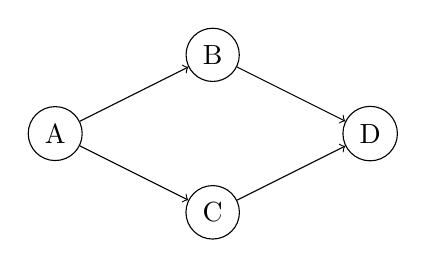
\begin{tikzpicture}
    \node[circle, draw] (A) at (0, 0) {A};
    \node[circle, draw] (B) at (2, 1) {B};
    \node[circle, draw] (C) at (2, -1) {C};
    \node[circle, draw] (D) at (4, 0) {D};

    \draw[->] (A) -- (B);
    \draw[->] (A) -- (C);
    \draw[->] (B) -- (D);
    \draw[->] (C) -- (D);
\end{tikzpicture}
\caption{有向グラフの図}
\end{centering}
\end{figure}

\subsection*{有向グラフの隣接行列}
\[
A = \begin{bmatrix}
0 & 1 & 1 & 0 \\
0 & 0 & 0 & 1 \\
0 & 0 & 0 & 1 \\
0 & 0 & 0 & 0 \\
\end{bmatrix}
\]

\subsection*{有向グラフの隣接リスト}
\begin{itemize}
    \item $ A: \rightarrow B \rightarrow C $
    \item $ B:\rightarrow D $
    \item $ C:\rightarrow D $
    \item $ D: \rightarrow $
\end{itemize}

\section*{問 2}
問題: グラフが同型であるとはどういうことか説明し、同型な2つのグラフの例を挙げよ.

模範解答:
グラフが同型であるとは、頂点の対応関係が存在し、辺の接続関係が保たれることを意味する.同型な2つのグラフの例として、グラフは以下となる.

\begin{figure}
\begin{centering}
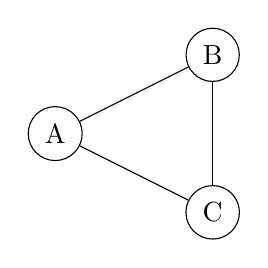
\begin{tikzpicture}
    \node[circle, draw] (A) at (0, 0) {A};
    \node[circle, draw] (B) at (2, 1) {B};
    \node[circle, draw] (C) at (2, -1) {C};

    \draw (A) -- (B);
    \draw (A) -- (C);
    \draw (B) -- (C);
\end{tikzpicture}
\caption{同型なグラフの図A}
\end{centering}
\end{figure}
\hspace{2cm}
\begin{figure}
\begin{centering}
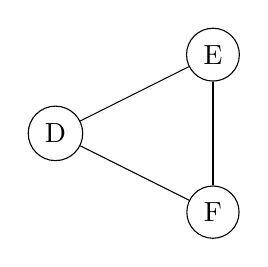
\begin{tikzpicture}
    \node[circle, draw] (D) at (0, 0) {D};
    \node[circle, draw] (E) at (2, 1) {E};
    \node[circle, draw] (F) at (2, -1) {F};

    \draw (D) -- (E);
    \draw (D) -- (F);
    \draw (E) -- (F);
\end{tikzpicture}
\caption{同型なグラフの図B}
\end{centering}
\end{figure}

\section*{問 3}
問題: グラフの次数について説明し、与えられたグラフの各頂点の次数を求めよ.

模範解答:
グラフの次数とは、ある頂点に接続されている辺の数を指す。グラフは以下となる.

\begin{figure}
\begin{centering}
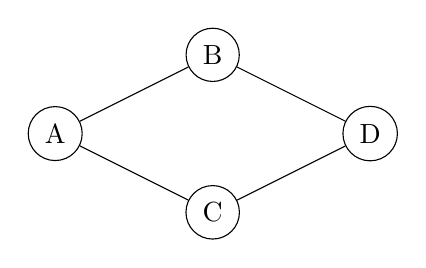
\begin{tikzpicture}
    \node[circle, draw] (A) at (0, 0) {A};
    \node[circle, draw] (B) at (2, 1) {B};
    \node[circle, draw] (C) at (2, -1) {C};
    \node[circle, draw] (D) at (4, 0) {D};

    \draw (A) -- (B);
    \draw (A) -- (C);
    \draw (B) -- (D);
    \draw (C) -- (D);
\end{tikzpicture}
\caption{問題のために与えられたグラフ}
\end{centering}
\end{figure}

\textbf{各頂点の次数:}
\begin{itemize}
    \item A: 2
    \item B: 2
    \item C: 2
    \item D: 2
\end{itemize}

\section*{問 4}
問題: 小道、道、回路、閉路の違いについて説明し、それぞれの違いを挙げよ.

模範解答:
\begin{itemize}
    \item 小道: 頂点を重複せずに訪れる道。
    \item 道: 辺を重複せずに訪れる道。
    \item 回路: 始点と終点が同じで、頂点を重複しない道。
    \item 閉路: 始点と終点が同じで、辺を重複しない道。
\end{itemize}

\begin{figure}
\begin{centering}
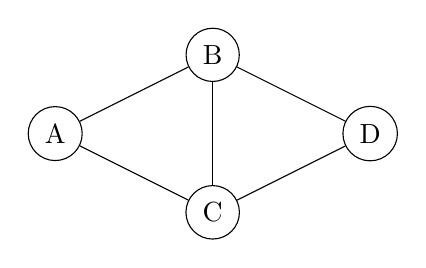
\begin{tikzpicture}
    \node[circle, draw] (A) at (0, 0) {A};
    \node[circle, draw] (B) at (2, 1) {B};
    \node[circle, draw] (C) at (2, -1) {C};
    \node[circle, draw] (D) at (4, 0) {D};

    \draw (A) -- (B);
    \draw (A) -- (C);
    \draw (B) -- (D);
    \draw (C) -- (D);
    \draw (B) -- (C); % This creates a cycle
\end{tikzpicture}
\caption{問題説明のためのグラフ}
\end{centering}
\end{figure}

\textbf{例:}
\begin{itemize}
    \item 小道: A $\to$ B $\to$ D
    \item 道: A $\to$ B $\to$ C $\to$ D
    \item 回路: A $\to$ B $\to$ C $\to$ A
    \item 閉路: B $\to$ C $\to$ D $\to$ B
\end{itemize}

\section*{問 5}
問題: 連結グラフの定義を述べ、連結グラフの例を示せ.

模範解答:
連結グラフとは、任意の2つの頂点間に道が存在するグラフを指す。グラフを以下とする.

\begin{figure}
\begin{centering}
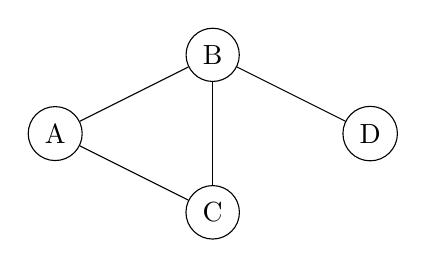
\begin{tikzpicture}
    \node[circle, draw] (A) at (0, 0) {A};
    \node[circle, draw] (B) at (2, 1) {B};
    \node[circle, draw] (C) at (2, -1) {C};
    \node[circle, draw] (D) at (4, 0) {D};

    \draw (A) -- (B);
    \draw (A) -- (C);
    \draw (B) -- (C);
    \draw (B) -- (D);
\end{tikzpicture}
\caption{連結グラフの図}
\end{centering}
\end{figure}

\section*{問 6}
問題: オイラー回路とハミルトン閉路の違いを説明し、それぞれの例を挙げよ.

模範解答:
オイラー回路とは、すべての辺を1回だけ通る閉路で、すべての頂点の次数が偶数である必要がある.ハミルトン閉路は、すべての頂点を1回だけ通る閉路のことである.

\begin{figure}
\begin{centering}
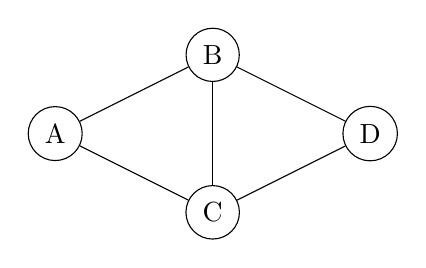
\begin{tikzpicture}
    \node[circle, draw] (A) at (0, 0) {A};
    \node[circle, draw] (B) at (2, 1) {B};
    \node[circle, draw] (C) at (2, -1) {C};
    \node[circle, draw] (D) at (4, 0) {D};

    \draw (A) -- (B);
    \draw (A) -- (C);
    \draw (B) -- (D);
    \draw (C) -- (D);
    \draw (B) -- (C); % This creates an Eulerian circuit
\end{tikzpicture}
\caption{オイラー回路}
\end{centering}
\end{figure}
\hspace{1cm}
\begin{figure}
\begin{centering}
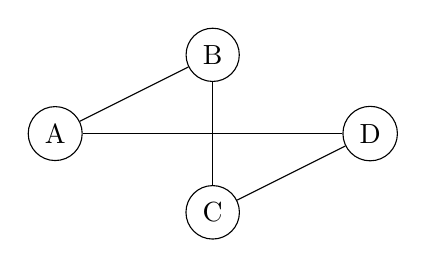
\begin{tikzpicture}
    \node[circle, draw] (A) at (0, 0) {A};
    \node[circle, draw] (B) at (2, 1) {B};
    \node[circle, draw] (C) at (2, -1) {C};
    \node[circle, draw] (D) at (4, 0) {D};

    \draw (A) -- (B);
    \draw (B) -- (C);
    \draw (C) -- (D);
    \draw (D) -- (A);
\end{tikzpicture}
\caption{ハミルトン閉路}
\end{centering}
\end{figure}

オイラー回路の例: 上のグラフはオイラー回路を持っている.

ハミルトン閉路の例: 下のグラフはハミルトン閉路を持っている.

\end{document}
